\chapter{စက်ရုပ်ကားရဲလ်ဖြင့် ပရိုဂရမ်းမင်းမိတ်ဆက်} \label{ch:ch01}
ကွန်ပျူတာတွေဟာ သက်မဲ့ စက်ပစ္စည်းတွေပါပဲ။ ကားတို့၊ လေယာဉ်တို့နဲ့ မတူတာက ကွန်ပျူတာတွေဟာ စက်ချည်းသက်သက် ဘာအစွမ်းမှ မယ်မယ်ရရ မရှိဘူး။ ဒါပေမဲ့ ဆောင်ရွက်လိုတဲ့ ကိစ္စအဝဝအတွက် ပရိုဂရမ်အမျိုးမျိုး ထည့်ပေးလိုက်တဲ့အခါမှာ သူ့ရဲ့အစွမ်းက အတိုင်းအဆမဲ့ပဲ။ နေရာမျိုးစုံ၊ နယ်ပါယ်မျိုးစုံမှာ အကူအညီပေးနိုင်တဲ့ စွယ်စုံသုံး ပစ္စည်းတစ်ခုဖြစ်သွားတယ်။ ဂီတသံစဉ်တွေကို ဖွင့်ပေးနိုင်သလို အသံလည်းသွင်းပေးနိုင်တယ်။ ရုပ်ရှင်တည်းဖြတ် လုပ်ချင်တာလား။ ပြဿနာမရှိဘူး၊ ကူညီပေးနိုင်တယ်။ နျူကလီး\allowbreak ယား ဓါတ်ပေါင်းဖိုတွေကို စီမံနိုင်သလို မောင်းသူမဲ့ ဒုံးပျံတွေကိုလည်း ပဲ့ထိန်းပေးနိုင်တယ်။ 

ကျွန်တော်တို့တွေ နိစ္စဓူဝ အသုံးပြုနေကြတဲ့ ကား၊ စမတ်ဖုန်း၊ လက်ပါတ်နာရီ၊ မိုက်ခရိုဝေဖ့်မီးဖို၊ အဝတ်လျှော်စက် စတဲ့ စက်ပစ္စည်း အမျိုးမျိုးဟာလည်း ကွန်ပျူတာတွေနဲ့ မကင်းပြန်ပါဘူး။ “ကွန်ပျူတာနည်းပညာ အကူအညီမပါတဲ့ ခေတ်မီဆန်းသစ်တီထွင်မှုဆိုတာ မရှိဘူး” လို့ ဆိုနိုင်ပါတယ်။

တစ်ချက်တစ်ချက် ရိုက်ခတ်လိုက်တဲ့ ကွန်ပျူတာနည်းပညာ လှိုင်းလုံးကြီးတွေဟာ ကမ္ဘာတစ်ဝှမ်းလုံး ပုံစံပြောင်းသွားလောက်အောင် အဟုန်ပြင်းထန်လှတယ်။ ဘီလီယံနဲ့ချီတဲ့ လူတွေ ဆိုရှယ်မီဒီယာတွေပေါ်ကနေ ရုပ်သံတွေနဲ့ ချိတ်ဆက်ပြောဆိုဆက်သွယ်လို့ ရစေတာဟာလည်း ကွန်ပျူတာစနစ်တွေပါပဲ။ \fEn{Artificial Intelligence (AI)} နည်းပညာကြောင့် သက်ရှိတွေမှာပဲတွေ့ရတဲ့ ညာဏ်ရည်မျိုးကို ကွန်ပျူတာတွေမှာလည်း တွေ့လာရပါပြီ။ သင်္ချာပုစ္ဆာတွေ ဖြေရှင်းခြင်း၊ စစ်တုရင်ထိုးခြင်း စတဲ့ကိစ္စမျိုးတွေအပြင် ပန်းချီဆွဲခြင်း၊ ကဗျာရေးစပ်ခြင်း၊ သီချင်းရေးဖွဲ့ခြင်း ကဲ့သို့ အနုပညာဖန်တီးမှုတွေကိုပါ \fEn{AI} က လုပ်ဆောင်ပေးနိုင်ပါတယ်။ နှစ်ဆယ့်တစ်ရာစုရဲ့ အထူးခြားဆုံး \fEn{AI} နည်းပညာလှိုင်းဟာ အရှိန်အဟုန်ပြင်းပြင်း ရိုတ်ခတ်ဖို့ အားယူစ ပြုနေပါပြီ။

‘ကွန်ပျူတာ’ လို့ပြောတဲ့အခါ စက်ပစ္စည်းသက်သက် မဟုတ်ဘဲ ကွန်ပျူတာမှတ်ညာဏ်ထဲက ပရိုဂရမ်တွေလည်း ပါဝင်တယ်ဆိုတာ သတိချပ်ရပါမယ်။ ကွန်ပျူတာတွေ တစ်စုံတစ်ရာ စွမ်းဆောင်နိုင်စေတဲ့  ပရိုဂရမ်တွေ ရေးတဲ့အလုပ်ကို ပရိုဂရမ်းမင်း \fEn{(Programming)} လို့ခေါ်တယ်။

\section{စက်ရုပ် ကားရဲလ်}
% ====================
ပရိုဂရမ်းမင်းဆိုတာ ဘယ်လိုမျိုးလဲ သဘောပေါက်အောင် စာတွေတစ်သီကြီးရေး ရှင်းပြတာထက် ပရိုဂရမ်လေးတွေ လက်တွေ့ ရေးကြည့်လိုက်တာ ပိုပြီးထိရောက်ပါတယ်။ ဒါကြောင့် စက်ရုပ်ကားရဲလ်ကို ပရိုဂရမ်လေးတွေရေးပြီး အလုပ်တွေခိုင်းကြည့်ကြမယ်။ ပုံ (\fRefNo{\ref{fig:meet_karel_1}}) မှာ တွေ့ရတာက ကားရဲလ် ရောက်ရှိနေတဲ့ နမူနာ ကမ္ဘာတစ်ခုပါ။ မီးခိုးရောင် မှန်ကူကွက်ပုံလေးကို ဘိပါ \fEn{(beeper)} လို့ ခေါ်တယ်။ အဲဒီဘိပါကို မြှားပြထားတဲ့ နေရာကို ရွှေ့ခိုင်းချင်တယ်။ မျဉ်းမည်းအထူတွေက နံရံတွေပါ။
%
\begin{figure}[htb!]
\begin{tikzonimage}[width=4in]{images/ch_a_programming_with_karel/meet_karel.jpg} %, tsx/show help lines]
    \draw[-{Latex[length=3mm]}] (0.7 ,0.8)--(0.645, 0.635);
\end{tikzonimage}
\caption{စက်ရုပ်လေး ကားရဲလ်}
\label{fig:meet_karel_1}
\end{figure}
%
ကားရဲလ်ကို ကိစ္စတစ်ခု ဆောင်ရွက်စေချင်တဲ့အခါ အခြေခံ ကားရဲလ်ကွန်မန်းတွေကို အသုံးပြုရပါတယ်။ ကွန်မန်းတွေကို နှုတ်နဲ့ပြောပြီး ခိုင်းရတာမဟုတ်ဘဲ ပရိုဂရမ်ရေးပြီး ခိုင်းရတာပါ။ ကားရဲလ်နားလည်တဲ့ ကွန်မန်းတွေကို ကြည့်ကြရအောင်။
%
\subsection*{ကားရဲလ်ကွန်မန်းများ}
% ==========================
မဖြစ်မနေ သိထားရမဲ့ အခြေခံ ကားရဲလ်ကွန်မန်း လေးခုပဲ ရှိတယ်။ \fCode{move}\fEn{,} \fCode{turn\_left}\fEn{,} \fCode{put\_beeper} နဲ့ \fCode{pick\_beeper}\ တို့ဖြစ်တယ်။ အခြား ကားရဲလ်ကွန်မန်း တွေလည်း ရှိပါသေးတယ်။ ဒါပေမဲ့ ကားရဲလ် ပရိုဂရမ်းမင်း စလေ့လာဖို့ ဒီလေးခုနဲ့ပဲ လုံလောက်ပါပြီ။

\fCode{move} ကွန်မန်းက ကားရဲလ်ကို ရှေ့တစ်ကွန်နာကို ရွှေ့ခိုင်းတာ။ ကားရဲလ်ကမ္ဘာထဲမှာ တစ်ခုနဲ့တစ်ခု အကွာအဝေးတူ ခြားထားတဲ့ အတန်းလိုက် အတန်းလိုက် အစက်ကလေးတွေဟာ ကွန်နာ \fEn{(corner)} တွေ ဖြစ်တယ်။ ကမ္ဘာကို မျဉ်းမည်းအထူ နံရံတွေနဲ့ ထောင့်မှန်စတုဂံပုံ ပါတ်လည် ဘောင်ခတ်ထားတယ်။ ကွန်နာတွေကြားမှာလည်း နံရံတွေရှိနိုင်တယ်။ နမူနာကမ္ဘာမှာ ဘေးတိုက် နံပါတ်စဉ် ၄ နဲ့ ၅ ကြား ထောင်လိုက် နံရံတစ်ခု၊ အထက်အောက် နံပါတ်စဉ် ၂ နဲ့ ၃ ကြား အလျားလိုက် နံရံတစ်ခုကို တွေ့ရပါမယ်။ ကွန်နာရှေ့မှာ နံရံကာနေရင် ကားရဲလ်ကို \fCode{move} ခိုင်းလို့မရပါဘူး။ 

\fCode{put\_beeper}\ က ကားရဲလ် လက်ရှိ ရှိနေတဲ့ ကွန်နာမှာ ‘ဘိပါတစ်ခုချ’ ထားခိုင်းတာ၊ \fCode{pick\_beeper}\ က ရပ်နေတဲ့ ကွန်နာမှာ ‘ဘိပါတစ်ခုကောက်’ ခိုင်းတာပါ။ ကွန်နာမှာ ဘိပါရှိနေမှ ကောက်ခိုင်းလို့ရမှာပါ။ မရှိရင် ကောက်ခိုင်းလို့ မရဘူး။ ဘိပါချခိုင်းရင်လည်း ကားရဲလ်မှာ ဘိပါရှိမှ ချခိုင်းလို့ရတယ်။ ကားရဲလ်ကို ဘိပါတွေ လိုသလောက် ဖြည့်ပေးထားတယ်လို့ ယူဆပါ။  \fCode{turn\_left} က ‘ဘယ်လှည့်’ ခိုင်းတာ။ \todo{ကမ္ဘာအသစ်တည်ဆောက်ရင် ဘိပါအရေအတွက် လိုသလိုဖြည့်ထားလို့ရကြောင်း ရှင်းပြဖို့လိုမလား}

\subsection*{ဘိပါကို ဘယ်လိုရွှေ့ခိုင်းမလဲ}
% ================================
ပုံ (\fRefNo{\ref{fig:meet_karel_1}}) အနေအထားကနေ ရှေ့ကို သုံးနေရာရွှေ့၊ ဘိပါကောက်၊ ဘယ်ဘက်လှည့်၊ အပေါ် နှစ်နေရာရွှေ့၊ ညာဘက်လှည့်၊ ရှေ့တစ်နေရာထပ်ရွှေ့ပြီး ဘိပါချထားခိုင်းလိုက်ရင် အလုပ်ပြီးသွားပါပြီ။

ကားရဲလ်ကို ညာဘက်လှည့်ခိုင်းဖို့ \fCode{turn\_right} ကွန်မန်း မရှိဘူး။ ဒါပေမဲ့ ဘယ်သုံးခါလှည့်တာဟာ ညာဘက်လှည့်တာနဲ့ တူတူပါပဲ။ ဒါကြောင့် ညာဘက်ချင်တဲ့အခါ ဘယ်သုံးခါလှည့်ခိုင်းလို့ရတယ်။

\section{Meet Karel ပရိုဂရမ်}
ပရိုဂရမ် ရေးတယ်ဆိုတာ ကွန်ပျူတာကို ကိစ္စတစ်ခုခု ဆောက်ရွက်ပေးဖို့ ခိုင်းစေတဲ့  ညွှန်ကြားချက်တွေ ရေးတာပါပဲ။ ဒီလို ညွှန်ကြားချက်တွေကို ပရိုဂရမ်ကုဒ် \fEn{(\textit{program code})} လို့ ခေါ်တယ်။ ပရိုဂရမ်ကုဒ်တွေကို ကွန်ပျူတာနားလည်တဲ့ \fEn{programming language} တစ်ခုခုနဲ့ ရေးရတယ်။ ဒီစာအုပ်မှာ အသုံးပြုမဲ့ \fEn{programming language} ကတော့ \fEn{Python} ပါ။ \fEn{Programming language} တစ်မျိုးပဲ ရှိတာမဟုတ်ပါဘူး။ ရာနဲ့ချီပြီး ရှိတာပါ။ လူ့ဘာသာစကားတွေ အမျိုးမျိုးရှိသလိုပဲပေါ့။ \fEn{Python} ဟာ ဒီလို ရာနဲ့ချီတဲ့ထဲက လက်ရှိအသုံးအများဆုံး ထိပ်ဆုံးဆယ်ခု ထဲမှာ ပါဝင်တယ်။ \fEn{Python} နဲ့ ဘိပါရွှေ့ခိုင်းတဲ့ ပရိုဂရမ်ကို လေ့လာကြည့်ရအောင်။ ကားရဲလ်နဲ့ ပထမဆုံး မိတ်ဆက်ပေးတဲ့ ပရိုဂရမ်မို့လို့ ဒီပရိုဂရမ် နံမည်ကို \fEn{‘Meet Karel’} လို့ ခေါ်ပါမယ်။
%
\setlength{\fboxsep}{0pt}
\begin{minted}[frame=\mintframe, framerule=\mintrule,framesep= \mintsep, xleftmargin=\xlftmargin
    , bgcolor=mintbgcolor,rulecolor=mintrulecolor
    , python3=true,escapeinside=ßß]{python}
# File: meet_karel.py
# About: This is
from stanfordkarel import *


def main():
    """Karel code goes here!"""
    move()
    move()
    move()
    pick_beeper()
    turn_left()
    move()
    move()

    turn_left()
    turn_left()
    turn_left()

    move()
    put_beeper()
# End of main

if __name__ == "__main__":
    run_karel_program("meet_karel")

\end{minted}
%

ဒါဟာ \fEn{‘Meet Karel’} ပရိုဂရမ်အတွက် \fEn{Python} နဲ့ရေးထားတဲ့ ပရိုဂရမ်ကုဒ် တွေဖြစ်ပါတယ်။ ‘\fEn{Python} ကုဒ်’ လို့ အတိုချုံးပဲ ပြောတာများတယ်။ \fEn{Python} ‘စာ/စကား’ မတတ်ရင် ဒီ ‘\fEn{Python} ကုဒ်’ တွေကိုလည်း နားလည်မှာ မဟုတ်ဘူး။ ဒီတော့ \fEn{Python} ‘စာ/စကား’ အခြေခံက စပြီး လေ့လာဖို့ လိုပါမယ်။
\todo{စာ ကို footnote ထည့်ရန်}

\subsection*{ကွန်းမန့် (Comment)}
ပထမဆုံး \fCode{\textit{\#}} သင်္ကေတနဲ့ စတဲ့ စာကြောင်းတွေက ကွန်းမန့်တွေပါ။ ကွန်းမန့်တွေက ကွန်ပျူတာ ဆောင်ရွက်ပေးရမဲ့ ညွှန်ကြားချက်တွေ မဟုတ်ဘူး။ ပရိုဂရမ်ကုဒ်နဲ့ ပါတ်သက်ပြီး ကုဒ် ဖတ်ရှူသူ အတွက် မှတ်ချက်ရေးတာ သို့မဟုတ် ရှင်းပြထားတာပါ။ တနည်းအားဖြင့် ဖတ်ရှုသူ (လူ) ပရိုဂရမ်မာအတွက် ရည်ရွယ်တာ။ ကွန်ပျူတာ (စက်) အတွက် ရည်ရွယ်တာ မဟုတ်ဘူး။ ကွန်ပျူတာက ကုဒ်ထဲက ကွန်းမန့်တွေ အားလုံးကို လစ်လျူရှုမှာပါ။ ဒါပေမဲ့ ပရိုဂရမ်ကုဒ်ကို ဖတ်တဲ့လူ နားလည်ဖို့ အထောက်အကူ ဖြစ်စေတဲ့အတွက် ကွန်းမန့်ရေးတာကို ပေါ့ပေါ့တန်တန် အရေးမပါသလို သဘောထားလို့ မရပါဘူး။ မိမိရေးတဲ့ ကုဒ်ကို ရှင်းပြဖို့ လိုအပ်ရင် ကွန်းမန့်ရေးရပါမယ်။ ရေးသင့်တဲ့ နေရာတွေကိုလည်း မကြာခင်တွေ့ရမှာပါ။

\subsection*{\fSubSecCodeBf{import} စတိတ်မန့်}
%
\setlength{\fboxsep}{0pt}
\begin{minted}[frame=\mintframe, framerule=\mintrule,framesep= \mintsep, xleftmargin=\xlftmargin
    , bgcolor=mintbgcolor,rulecolor=mintrulecolor
    , python3=true,escapeinside=ßß]{python}
from stanfordkarel import *
\end{minted}
%
ကတော့ အင်ပို့စတိတ်မန့် ဖြစ်ပါတယ်။ “\fCode{stanfordkarel} လိုက်ဘရီမှ အာလုံးကို ထည့်သွင်းပေးပါ” လို့ တောင်းဆိုတဲ့ အဓိပ္ပါယ်။ \fCode{*} သင်္ကေတကို ‘အားလုံး’ လို့ ယူဆပါ။  \fCode{stanfordkarel} လိုက်ဘရီမှာ ကားရဲလ်ပရိုဂရမ်အတွက် လိုအပ်တာအားလုံး   ပါဝင်တယ်။  ဒီလိုက်ဘရီကို အင်ပို့လုပ်ထားမှ ကားရဲလ်ကွန်မန်းတွေ သုံးလို့ရမှာပါ။ သီးခြား ကားရဲလ်ပရိုဂရမ် တစ်ခုစီတိုင်းအတွက် အင်ပို့လုပ်ရမှာ ဖြစ်တယ်။

\subsection*{လိုက်ဘရီ}
လိုက်ဘရီ \fEn{(\textit{library})} ဆိုတာ ပညာရပ်နယ်ပယ် တစ်ခုအတွက် ရည်ရွယ်ရေးထားတဲ့ ပရိုဂရမ်ကုဒ်တွေပါပဲ။ သင်္ချာအတွက်အချက် လိုက်ဘရီ၊ ဂိမ်းရေးဖို့ လိုက်ဘရီ၊ \fEn{2D/3D} ဂရပ်ဖစ်ဆွဲဖို့ လိုက်ဘရီ၊ အေအိုင်အတွက် လိုက်ဘရီ စသည်ဖြင့် နယ်ပယ်အသီးသီး၊ ကိစ္စရပ်အဖုံဖုံအတွက် သက်ဆိုင်ရာ ကျွမ်းကျင်ပညာရှင်တွေ ထုတ်လုပ်ဖြန့်ချီပေးထားတဲ့ လိုက်ဘရီတွေရှိတယ်။ \fEn{Matrix} အော်ပရေးရှင်းတွေအတွက် \fCode{numpy} ၊ ဂရပ်ဖ်ဆွဲမယ်ဆိုရင် \fCode{matplotlib} စတဲ့ လိုက်ဘရီတွေကို အင်ပို့လုပ် အသုံးပြုနိုင်ပါတယ်။ မေ့ထရစ် $A$ ကို $B$ နဲ့ မြှောက်ရင် ဒီလိုပါ 
%
\setlength{\fboxsep}{0pt}
\begin{minted}[frame=\mintframe, framerule=\mintrule,framesep= \mintsep, xleftmargin=\xlftmargin
    , bgcolor=mintbgcolor,rulecolor=mintrulecolor
    , python3=true,escapeinside=ßß]{python}
from numpy import *

A = array([[1, 1, 2, 2],
           [2, 2, 1, 1],
           [2, 2, 1, 1]])
B = array([[2, 2],
           [2, 2],
           [1, 1],
           [2, 2]])

result = matmul(A, B)

print(result)

\end{minted}
%
ရလဒ် အခုလိုထွက်ပါမယ်။ 
%
\begin{minted}[frame=lines, framerule=0pt]{text}
[[10 10]
 [11 11]
 [11 11]]
\end{minted}
%
ဒါကတော့ ဘားချတ် အတွက် \fCode{numpy} နဲ့ \fCode{matplotlib} လိုက်ဘရီ သုံးထားတာပါ။  
%
\setlength{\fboxsep}{0pt}
\begin{minted}[frame=\mintframe, framerule=\mintrule,framesep= \mintsep, xleftmargin=\xlftmargin
    , bgcolor=mintbgcolor,rulecolor=mintrulecolor
    , python3=true,escapeinside=ßß]{python}
from matplotlib.pyplot import *
from numpy import *

# make data:
x = 0.5 + arange(8)
y = [4.8, 5.5, 3.5, 4.6, 6.5, 6.6, 2.6, 3.0]

# plot
fig, ax = subplots()
bar(x, y, width=1, edgecolor="white", linewidth=0.7)

ax.set(xlim=(0, 8), xticks=arange(1, 8),
       ylim=(0, 8), yticks=arange(1, 8))

show()
\end{minted}
ဘားချတ်ကို ဒီလို ထုတ်ပေးပါတယ်။
%
\begin{figure}[tbh!]
\begin{tikzpicture}
    \node[anchor=south west,inner sep=0] (image) at (0,0)
        {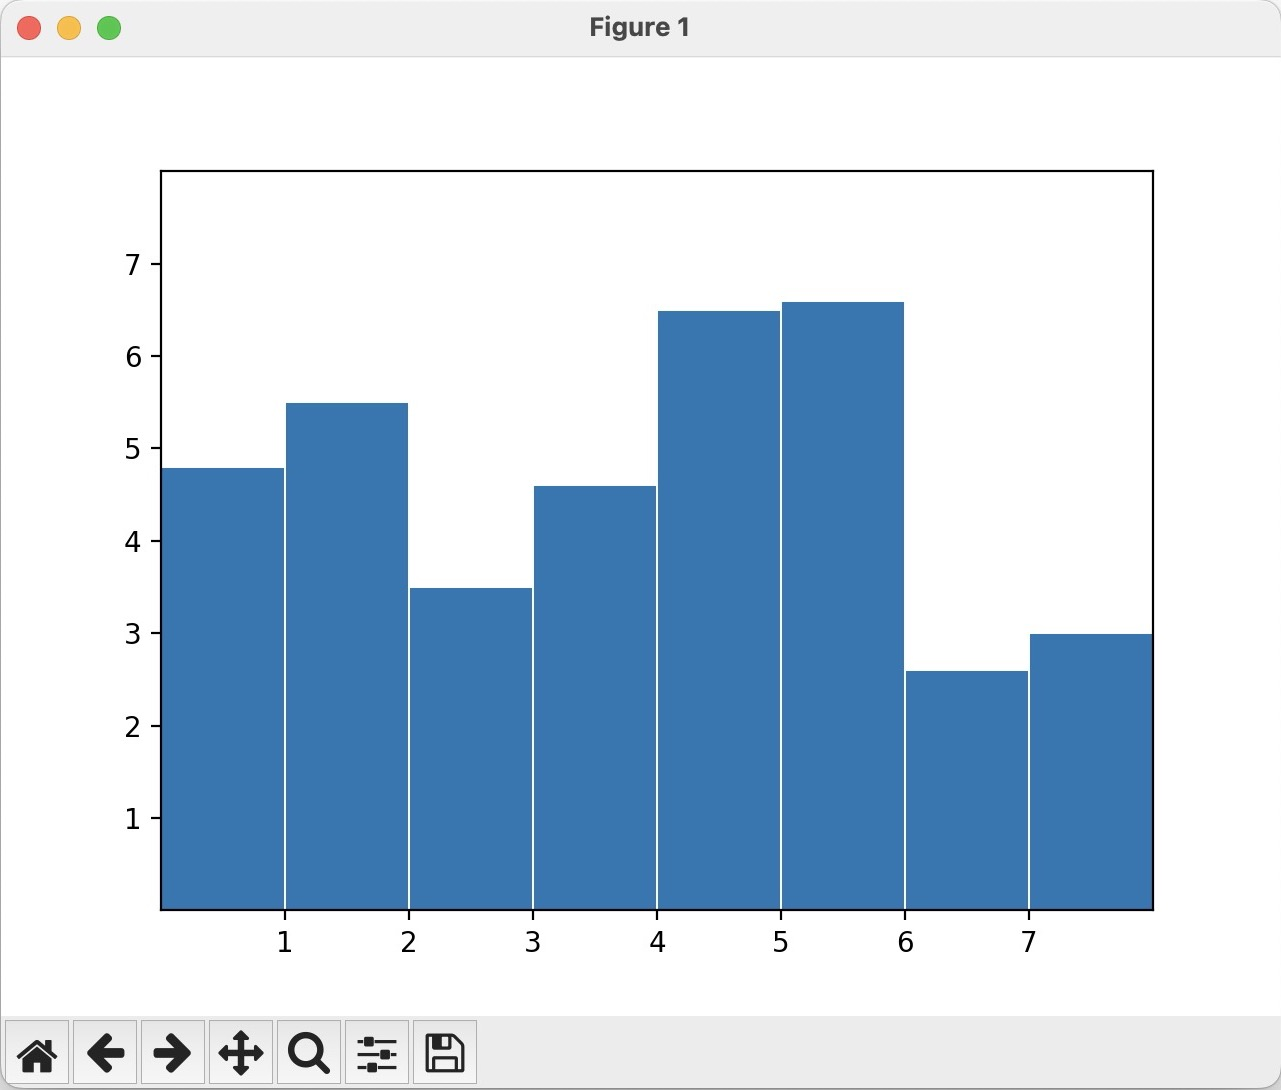
\includegraphics[width=.5\textwidth, trim={2.4mm 2mm 2mm 2mm},clip]{images/ch01/bar.jpg}};
    \drawshadow{image}
\end{tikzpicture}
\caption{} 
\label{fig:}
\end{figure}

လိုက်ဘရီတွေဟာ ပရိုဂရမ်တွေ တည်ဆောက်ရာမှာ အင်မတန်မှ အရေးပါတယ်။ ဖော်ပြထားတဲ့ မေ့ထရစ် နဲ့ ဘားချတ်  ကုဒ်တွေကို (အခုတော့) နားလည်မှာ မဟုတ်သေးဘူးပေါ့။ ဒါပေမဲ့ သက်ဆိုင်ရာ လိုက်ဘရီတွေနဲ့ ဒီလိုကိစ္စတွေကို သိပ်မခက်ခဲဘဲ လုပ်လို့ရနိုင်တယ်ဆိုတာ မြင်မယ် ထင်ပါတယ်။ လိုက်ဘရီတွေသာမရှိရင် ပရိုဂရမ်တွေကို အခုထက် အဆပေါင်းများစွာ အချိန်ပေးပြီး ရှုပ်ရှုပ်ထွေးထွေး ခက်ခက်ခဲခဲ တည်ဆောက်ကြရမှာပါ။ 


\subsection*{တုံကင်၊ စတိတ်မန့်နှင့် ဆင်းတက်စ်}
ဂျန်ပန်စာ၊ ပြင်သစ်စာ စတဲ့ လူ့ဘာသာစကားတွေဟာ  စကားလုံးတွေ ဝါကျတွေနဲ့ ဖွဲ့စည်းထားသလို ပရိုဂရမ်ကုဒ်တွေဟာလည်း စကားလုံးတွေ၊ ဝါကျတွေနဲ့ ဖွဲ့စည်းထားတာပါပဲ။ \fEn{Programming language} တွေမှာ စကားလုံးတွေကို တုံကင် \fEn{(\textit{token})} လို့ခေါ်ပြီး  ဝါကျတွေကိုတော့ စတိတ်မန့် \fEn{(\textit{statement})} လို့ ခေါ်ပါတယ်။ ဝါကျတွေကို စကားလုံးတွေနဲ့ ဖွဲ့စည်းထားသလို စတိတ်မန့်တွေကတော့ တုံကင်တွေနဲ့ ဖွဲ့စည်းထားတာပါ။ စတိတ်မန့် ပုံစံတစ်မျိုးကို တွေခဲ့ပြီးပါပြီ။ အဲဒါကတော့ ရှေ့စာမျက်နှာက အင်ပို့စတိတ်မန့်ပဲ ဖြစ်ပါတယ်။ 

လူ့ဘာသာစကားတွေမှာ ဖွဲ့စည်းတည်ဆောက်ပုံ စထရက်ချာရှိသလို \fEn{programming language} တွေမှာလည်း စထရက်ချာရှိဖို့ လိုအပ်တာပေါ့။  ဖွဲ့စည်းပုံ စထရက်ချာ မှန်/မမှန်ကို သဒ္ဒါစည်းမျဉ်တွေနဲ့ ထိန်းကွပ်ထားတာပါ။ ပရိုဂရမ်ကုဒ် စထရက်ချာ မှန်/မမှန် ထိန်းကွပ်ပေးတဲ့ သဒ္ဒါစည်းမျဉ်တွေကိုတော့ ဆင်းတက်စ် \fEn{(\textit{syntax})} လို့ခေါ်တယ်။

မြန်မာလိုရေးရင် မြန်မာသဒ္ဒါကို လိုက်နာရသလို \fEn{Python} နဲ့ ရေးရင် \fEn{Python} ဆင်းတက်စ်ကို လိုက်နာရမှာပေါ့။ မြန်မာသဒ္ဒါမှားရင် ဖတ်တဲ့သူက သည်းခံနားလည် ပေးပေမဲ့ ဆင်းတက်စ်မှားရင်တော့ \fEn{Python} က လုံးဝ လက်ခံမှာ မဟုတ်ပါဘူး။ ဆင်းတက်စ် စည်းကမ်းတွေဟာ ပိုပြီး တင်းကျပ်တယ်။ လွဲချော်လို့ မရဘူး။ ဆင်းတက်စ်မှားနေတဲ့ ပရိုဂရမ်ကို  \fEn{Python} က \fEn{run} ခွင့် ပြုမှာမဟုတ်ဘဲ အမှားနဲ့သက်ဆိုင်တဲ့ အယ်ရာ\fOpn{မက်ဆေ့ချ်}တွေ ပြပေးမှာပါ။ ဖြစ်လေ့ရှိတဲ့ ဆင်းတက်စ်အမှားတွေကို မကြာခင် တွေ့ရပါမယ်။

\subsection*{Keywords}
\fCode{from}\fEn{,} \fCode{import}\fEn{,} \fCode{def} \fEn{,} \fCode{if} စတာတွေဟာ \fEn{\textit{keyword}} တွေဖြစ်တယ်။ \fEn{Python} ရေးတဲ့အခါ သူ့နေရာနဲ့သူ အဓိပ္ပါယ်ကိုယ်စီနဲ့ အသုံးပြုရတဲ့ စကားလုံးတွေဖြစ်တယ်။ \fCode{from} နဲ့ \fCode{import} ကို လိုက်ဘရီ အင်ပို့လုပ်ဖို့ သုံးတယ်။ \fCode{def} ကို ဖန်ရှင် သတ်မှတ်တဲ့အခါ သုံးတယ်။ \fEn{Python} က သတ်မှတ်ထားတဲ့ နေရာတွေကလွဲလို့ အခြားကိစ္စတွေအတွက် \fEn{keyword} တွေကို အသုံးပြုလို့ မရပါဘူး။ ဒါကြောင့်  \fEn{keyword} တွေကို \fEn{reserved word} လို့လည်း ခေါ်တယ်။ 

\subsection*{\fSubSecCodeBf{main} ဖန်ရှင်}
\fEn{‘Meet Karel’} ပရိုဂရမ် အင်ပို့စတိတ်မန့် အပြီးမှာ တွေ့ရတာကတော့ \fCode{main} ဖန်ရှင်သတ်မှတ်ချက်ပါ။ ကြည့်ရအဆင်ပြေအောင် သူ့ချည်းသီးသန့် တစ်ဖြတ် ပြန်ပြပေးထားပါတယ်။
%
\setlength{\fboxsep}{0pt}
\begin{minted}[frame=\mintframe, framerule=\mintrule,framesep= \mintsep, xleftmargin=\xlftmargin
    , bgcolor=mintbgcolor,rulecolor=mintrulecolor
    , python3=true,escapeinside=ßß]{python}
def main():
    """Karel code goes here!"""
    move()
    move()
    move()
    pick_beeper()
    turn_left()
    move()
    move()

    turn_left()
    turn_left()
    turn_left()

    move()
    put_beeper()
# End of main
\end{minted}

\begin{mytcbox}
ဖန်ရှင် \fEn{(\textit{function})} ဆိုတာ ကိစ္စတစ်ခု လုပ်ဆောင်ပေးဖို့အတွက် ယူနစ်တစ်ခုအနေနဲ့ ဖွဲ့စည်းထားတဲ့ ပရိုဂရမ်ကုဒ် အစုအဝေးတစ်ခုပါပဲ။ ဖန်ရှင်ကို အသုံးပြုတဲ့အခါ ၎င်းရဲ့ လုပ်ငန်းတာဝန်အတိုင်း ဖန်ရှင်က လုပ်ဆောင်ပေးမှာ ဖြစ်တယ်။ ဖန်ရှင်အသုံးပြုတာကို ‘ဖန်ရှင်ကောလ်’  \fEn{(\textit{function call})} လုပ်တာလို့ ပြောတယ်။
\end{mytcbox}
%
\fCode{main} ဖန်ရှင်သတ်မှတ်ချက်ကို အပိုင်းနှစ်ပိုင်းခွဲ ကြည့်နိုင်တယ်။ ပထမတစ်ပိုင်း
%
\setlength{\fboxsep}{0pt}
\begin{minted}[frame=\mintframe, framerule=\mintrule,framesep= \mintsep, xleftmargin=\xlftmargin
    , bgcolor=mintbgcolor,rulecolor=mintrulecolor
    , python3=true,escapeinside=ßß]{python}
def main():
\end{minted}
%
ကို ဖန်ရှင်ခေါင်းစီး \fEn{(function header)} လို့ခေါ်တယ်။ ဖန်ရှင်ခေါင်းစီးမှာ ဖန်ရှင်နံမည်နဲ့ ဖန်ရှင်ပါရာမီတာတွေကို ဝိုက်ကွင်းထဲမှာ သတ်မှတ်ပေးရပြီး \fEn{colon} \fEn{‘\fCode{:}’}  နဲ့ အဆုံးသတ်တယ်။ ဥပမာ \fCode{x}\fEn{,} \fCode{y} ပါရာမီတာ နဲ့  \fCode{myfun} ဖန်ရှင် အတွက် 
%
\setlength{\fboxsep}{0pt}
\begin{minted}[frame=\mintframe, framerule=\mintrule,framesep= \mintsep, xleftmargin=\xlftmargin
    , bgcolor=mintbgcolor,rulecolor=mintrulecolor
    , python3=true,escapeinside=ßß]{python}
def myfun(x, y):
\end{minted}
ပါရာမီတာမပါရင်လည်း ဝိုက်ကွင်းအလွတ် တစ်စုံ \fEn{‘\fCode{()}’} တော့ပါရမယ်။ \fCode{main} ဖန်ရှင်မှာ ပါရာမီတာ မပါဘူး။ ပါရာမီတာတွေအကြောင်း နောက်ပိုင်းအခန်းတွေမှာ အသေးစိတ် လေ့လာရမှာပါ။ ကားရဲလ်ပရိုဂရမ်တွေမှာ ပါရာမီတာအကြောင်း သိဖို့မလိုသေးပါဘူး။ ပါရာမီတာ မလိုတဲ့ ဖန်ရှင်တွေပဲ တွေ့ရမှာပါ။ 

ဖန်ရှင်ခေါင်းစည်းအောက် ဒုတိယပိုင်းကတော့ \fCode{main} ဖန်ရှင် ကုဒ်ဘလောက် \fEn{(\textit{code block})} ပါ။ ကုဒ်ဘလောက် ဆိုတာ ကုဒ်တွေကို အုပ်စုတစ်စု အဖြစ် ဖွဲ့စည်းထားတာကို ဆိုလိုတာပါ။ ဘလောက်လို့လည်း ခေါ်တယ်။ ဘလောက်တစ်ခုမှာ ပါဝင်တဲ့ ကုဒ်လိုင်းတွေကို ညာဘက် ခွာရေးရပါမယ်။ အင်ဒန့်ထ် \fEn{(indent)} လုပ်တာလို့ ခေါ်တယ်။  တက်ဘ်ကီးတစ်ချက် (သို့) စပေ့စ်လေးခုစာ ခွာလေ့ရှိတယ်။  ဘော်ဒီ ပထမတစ်ကြောင်း
%ချိန်ညှိရေးထားတဲ့
\setlength{\fboxsep}{0pt}
\begin{minted}[frame=\mintframe, framerule=\mintrule,framesep= \mintsep, xleftmargin=\xlftmargin
    , bgcolor=mintbgcolor,rulecolor=mintrulecolor
    , python3=true,escapeinside=ßß]{python}
"""Karel code goes here!"""
\end{minted}
ကို \fEnEmp{docstring} လို့ ခေါ်တယ်။ \fEn{quote} သုံးခုတွဲ \fEn{‘\fCode{"""}’} တစ်စုံကြား ညှပ်ရေးတဲ့ ကွန်းမန့်တစ်မျိုးလို့ ယူဆနိုင်တယ်။ ဖန်ရှင်နဲ့ ပါတ်သက်တဲ့ ရှင်းလင်းဖော်ပြချက်တွေ ရေးဖို့အတွက် သုံးတာပါ။

\fEn{Docstring} အောက်မှာ တွေ့ရတာကတော့ ကားရဲလ်ကွန်မန်းတွေဆိုတာ သိပါလိမ့်မယ်။ ကားရဲလ်ကွန်းမန်းတွေဟာ \fCode{stanfordkarel} လိုက်ဘရီ ဖန်ရှင်တွေပါ။ တနည်းအားဖြင့် \fCode{stanfordkarel} လိုက်ဘရီမှာ ကားရဲလ်ကွန်းမန်းတွေအတွက် ဖန်ရှင်သတ်မှတ်ချက်တွေ ပါဝင်တယ်။ ဖန်ရှင်တစ်ခုကို အသုံးပြုဖို့အတွက် အဲဒီဖန်ရှင်ကို ခေါ်ရပါတယ်။ ဒါကို   ဖန်ရှင်ကောလ် \fEn{(\textit{function call})} လုပ်တယ်လို့ ပြောတယ်။ ကားရဲလ်ကို ဘယ်ဘက်လှည့်စေချင်ရင် \fCode{turn\_left} ဖန်ရှင်ကောလ် လုပ်ရပါမယ်။ ဘိပါကောက်ခိုင်းချင်ရင် \fCode{pick\_beeper} ဖန်ရှင်ကောလ် လုပ်ရပါမယ်။ ဖန်ရှင်ကောလ် လုပ်တဲ့ ပုံစံက
%
\setlength{\fboxsep}{0pt}
\begin{minted}[frame=\mintframe, framerule=\mintrule,framesep= \mintsep, xleftmargin=\xlftmargin
    , bgcolor=mintbgcolor,rulecolor=mintrulecolor
    , python3=true,escapeinside=ßß]{python}
turn_left()
pick_beeper()
\end{minted}
စသည်ဖြင့် ဖြစ်တယ်။

\begin{mytcbox}
\fEn{Python} မှာ အင်ဒန့်ထ်ကို ဖြစ်ကတတ်ဆန်း လုပ်လို့မရဘူး။ ဘေးမျဉ်းကနေ ခွာတဲ့ အကွာအဝေး မညီတာနဲ့ ဆင်းတက်စ်အမှား ဖြစ်တယ်။ မလိုတဲ့နေရာမှာလည်း ခွာရေးလို့ မရဘူး။ ခေါင်းစီးကို ဘေးမျဉ်းနဲ့ ခွာထားကြည့်ပါ။ အယ်ရာဖြစ်တာကို တွေ့ရမယ်။ အင်ပို့စတိတ်မန့်လည်း ဘေးမျဉ်းနဲ့ ကွာနေလို့မရဘူး။ အခြား \fEn{language} တွေမှားလည်း အင်ဒန့်ထ်လုပ် ရေးကြပေမဲ့ \fEn{Python} မှာလောက် မတင်းကျပ်ဘူး။ အင်ဒန့်ထ်မလုပ်လည်း ဆင်းတက်စ်မှားတာ မဖြစ်ဘူး။
\end{mytcbox}

ကားရဲလ်ပရိုဂရမ်တစ်ခုမှာ \fCode{main} ဟာ  အထူးတာဝန်တစ်ခု လုပ်ဆောင်ပေးရတယ်။ အဲဒါကတော့ ပရိုဂရမ်ဝင်းဒိုးမှာ \mytcboxinl{\fEnSnd{Run Program}}  ခလုတ် (ပုံ \fRefNo{\ref{fig:mtkrlprgm1}} မှာကြည့်ပါ) နှိပ်လိုက်ရင် တုံ့ပြန် လုပ်ဆောင်ပေးရတာပါ။ ဒါကြောင့် ကွန်မန်းတွေဟာ အဲဒီခလုတ် နှိပ်တော့မှပဲ စအလုပ်လုပ်တာ ဖြစ်တယ်။

\subsection*{Entry Point}
\fEn{‘Meet Karel’} ပရိုဂရမ်မှာ \fCode{main} ဖန်ရှင်နောက် အောက်ဆုံးအပိုင်းဟာ ပရိုဂရမ် \fEn{run} တဲ့အခါ ပထမဆုံး စတင်လုပ်ဆောင်ပေးရမဲ့ ဖန်ရှင်ကို ဖော်ပြပေးတာပါ။ အန်ထရီပွိုင့် \fEn{(\textit{entry point})} လို့ခေါ်တယ်။ 
%
\setlength{\fboxsep}{0pt}
\begin{minted}[frame=\mintframe, framerule=\mintrule,framesep= \mintsep, xleftmargin=\xlftmargin
    , bgcolor=mintbgcolor,rulecolor=mintrulecolor
    , python3=true,escapeinside=ßß]{python}
if __name__ == "__main__":
    run_karel_program("meet_karel")
\end{minted}
%
\fCode{run\_karel\_program} ဖန်ရှင်ဟာ ကားရဲပရိုဂရမ် တစ်ခုအတွက် အန်ထရီပွိုင့် ဖြစ်တယ်။  ပရိုဂရမ် တက်လာတာနဲ့ တစ်ပါတည်း ခေါ်တင်ချင်တဲ့ ကမ္ဘာကို ဒီဖန်ရှင်မှာ ထည့်ပေးတယ်။ \fEnSnd{meet\_karel.w} ကမ္ဘာကို စစချင်းခေါ်တင်ထားချင်ရင် \fCode{"meet\_karel"} ထည့်ပေးရမယ်။  ကမ္ဘာဖိုင်မရှိရင် အယ်ရာတက်ပြီး ပရိုဂရမ်ပွင့်လာမှာ မဟုတ်ဘူး။ ကမ္ဘာမထည့်ပေးထားဘဲ ဒီလို
%
\setlength{\fboxsep}{0pt}
\begin{minted}[frame=\mintframe, framerule=\mintrule,framesep= \mintsep, xleftmargin=\xlftmargin
    , bgcolor=mintbgcolor,rulecolor=mintrulecolor
    , python3=true,escapeinside=ßß]{python}
run_karel_program()
\end{minted}
%
ဆိုရင် $8 \times 8$ အရွယ် \fEn{default} ကမ္ဘာကို တင်ပေးပါတယ်။

ကားရဲလ်ကမ္ဘာတစ်ခုကို လိုချင်တဲ့ပုံစံ ဒီဇိုင်းဆွဲပြီး ဖိုင်နဲ့ သိမ်းထားရတာပါ။ ကမ္ဘာ ပုံစံချတဲ့ ပရိုဂရမ်လည်း ရှိတယ်။ ကမ္ဘာဖိုင်တွေက \fEnSnd{.w} ဖိုင် အိပ်စ်တန်းရှင်းနဲ့ ဖြစ်တယ်။ ဒီစာအုပ်မှာပါတဲ့ ဥပမာတွေ၊ လေ့ကျင့်ခန်းတွေ အားလုံးအတွက် လိုအပ်တဲ့ ကမ္ဘာတွေကို အဆင်သင့်ပေးထားမှာပါ။ ကိုယ့်ဟာကို လုပ်ဖို့ မလိုဘူး။ စိတ်ဝင်စားရင် စမ်းကြည့်လို့ရအောင် စာမျက်နှာ (\fRefNo{\pageref{apdx:02}}) နောက်ဆက်တွဲ (\fRefNo{\ref{apdx:02}}) မှာ အကျဉ်းဖော်ပြပေးထားပါတယ်။

\section{ကားရဲလ် ပရိုဂရမ် run ခြင်း}

လိုအပ်တဲ့ဆော့ဖ်ဝဲတွေ ထည့်သွင်းနည်းကို စာမျက်နှာ (\fRefNo{\pageref{apdx:01}}) နောက်ဆက်တွဲ (\fRefNo{\ref{apdx:01}}) မှာ တစ်ဆင့်ချင်း ဖော်ပြပေးထားပါတယ်။ အခုက \fEn{Python} ပရိုဂရမ်တစ်ခုကို အရိုးရှင်းဆုံး (လွယ်တယ်လို့ မဆိုလို)  \fEn{run} လို့ရတဲ့ နည်းကိုဖော်ပြပေးမှာပါ။ သဘောတရားပိုင်း နားလည်ဖို့ အထောက်အပံ့ဖြစ်မယ်။ အခုနည်းလမ်းကို အကြမ်းဖျဉ်း နားလည်အောင် ဖတ်ပြီးမှ နောက်ဆက်တွဲ (\fRefNo{\ref{apdx:01}}) ကို ဖတ်စေချင်ပါတယ်။

မိုက်ခရိုဆော့ဖ် ဝင်းဒိုးမှာ \fEn{Notepad} ၊ အက်ပဲလ် မက်ခ်အိုအက်စ်မှာ  \fEn{TextEdit} စတဲ့ တက်စ် အယ်ဒီတာတစ်ခုခုနဲ့ ပရိုဂရမ်ကုဒ်ရေးလို့ရတယ်။ ကုဒ်ဖိုင်ကို \fEnSnd{.py} အိပ်စ်တန်းရှင်းနဲ့ သိမ်းရပါမယ်။ ပလိန်းတက်စ် \fEn{(plain text)} ဖိုင် ပါပဲ။ \fEn{Python} ကုဒ်ဖိုင်မို့လို့ \fEnSnd{.txt} အစား \fEnSnd{.py} နဲ့ သိမ်းတာပါ။ \fEn{Python} ဖိုင် နံမည်ကို စာလုံးအသေးနဲ့ပဲ ပေးတဲ့ ထုံးစံရှိတယ်။  စပေ့စ်နေရာမှာ \fEnSnd{ \_} \fEn{(underscore)} သုံးတဲ့ ထုံးစံရှိတယ်။ ဒါကြောင့် \fEn{‘Meet Karel’} ပရိုဂရမ်ကုဒ်ကို \fEnSnd{meet\_karel.py} ဖိုင်မှာ သိမ်းသင့်တယ်။ 

\fEn{Python} နဲ့ ရေးထားတဲ့ ပရိုဂရမ်ကို \fEn{run} မယ်ဆိုရင် \fEn{Python} ဆော့ဖ်ဝဲရှိရမှာပါ။ ဒီဆော့ဖ်ဝဲ အင်စတောလ် လုပ်နည်းကို နောက်ဆက်တွဲ (\fRefNo{\ref{apdx:01}}) စာမျက်နှာ (\fRefNo{\pageref{subsec:pyinstl}}) မှာ ဖော်ပြပေးထားပါတယ်။ \fEn{Python} ကုဒ်တွေကို ကွန်ပျူတာက တိုက်ရိုက် နားမလည်ပါဘူး။ \fEn{Python} ဆော့ဖ်ဝဲဟာ \fEn{Python} ကုဒ်တွေကို တိုက်ရိုက် နားလည်ပြီး ကွန်ပျူတာပေါ်မှာ \fEn{run} လို့ရအောင် ကြားခံဆောင်ရွက်ပေးတဲ့ ဆော့ဖ်ဝဲလို့ ယေဘုယျအားဖြင့် ယူဆနိုင်တယ်။

\fEn{Python} ထည့်ပြီးရင် \fCode{stanfordkarel} လိုက်ဘရီကို အောက်ပါကွန်မန်းနဲ့ အင်စတောလ် လုပ်ရပါမယ်။ အင်တာနက်ပေါ်ကနေ ဒေါင်းလုဒ် လုပ်ရတာမို့လို့ ကွန်နက်ရှင်ရှိရမယ်။
%
\begin{minted}[frame=lines, framerule=0pt]{text}
pip install stanfordkarel
\end{minted}
%

ကားရဲလ်ပရိုဂရမ်မှာ ခေါ်တင်ချင်တဲ့ ကမ္ဘာဖိုင်တွေလည်း ရှိရပါမယ်။  \fEnSnd{meet\_karel.w} ကမ္ဘာဖိုင်က \fEnSnd{meet\_karel.zip} ဖိုင် \fEnSnd{worlds} ဖိုဒါထဲမှာ ရှိပါတယ်။  \fCode{http://tinyurl.com/3mmm9c7j} လင့်ကနေ \fEnSnd{meet\_karel.zip}  ဖိုင်ကို ဒေါင်းလုဒ်လုပ်ပါ။ ဒီ \fEnSnd{zip} ဖိုင်ထဲက \fEnSnd{worlds} ဖိုဒါကို \fEnSnd{meet\_karel.py} ဖိုင်ရှိတဲ့နေရာမှာ ကော်ပီကူးထည့်ပါ။ ဝင်းဒိုးမှာ \fEn{Command Prompt} ၊ မက်ခ်အိုအက်စ်မှာ  \fEn{Terminal} ဖွင့်ပြီး \fEnSnd{cd} ကွန်မန်းနဲ့ ကုဒ်ဖိုင်ထားတဲ့ ဖိုဒါထဲကို သွားပြီး အောက်ပါအတိုင်း \fEnSnd{python} ကွန်မန်းနဲ့ ကုဒ်ဖိုင်ကို \fEn{run} ပေးရပါမယ် (လာမဲ့စာမျက်နှာမှာ နမူနာပြထားတာ ကြည့်ပါ)။ 
%
\begin{minted}[frame=lines, framerule=0pt,escapeinside=ßß]{text}
python meet_karel.py
\end{minted}
ကုဒ်ရေးထားတာ ဆင်းတက်စ်အမှား မရှိဘူးဆိုရင် ကားရဲပရိုဂရမ် ပွင့်လာမှာပါ။

အခုဖော်ပြခဲ့တာက ကားရဲလ်ပရိုဂရမ်တစ်ခု \fEn{run} ဖို့ မဖြစ်မနေလုပ်ရမဲ့ အနည်းဆုံးလိုအပ်ချက်ပါ။ \fEn{Python} ဆော့ဖ်ဝဲ ရှိရမယ်။ \fCode{stanfordkarel} လိုက်ဘရီ အင်စတောလ် လုပ်ရမယ်။ ကမ္ဘာဖိုင်ပါတဲ့ \fEnSnd{worlds} ဖိုဒါရှိရမယ်။ \fEnSnd{.py} ဖိုင် တစ်ခုနဲ့ ပရိုဂရမ်ကုဒ်ကို သိမ်းရမယ်။ \fEnSnd{worlds} ဖိုဒါနဲ့ ကုဒ်ဖိုင်ကို တစ်နေရာတည်းမှာ ထားရမယ်။ ပြီးရင် ကွန်မန်းလိုင်းမှာ 
%
\begin{minted}[frame=lines, framerule=0pt,escapeinside=ßß]{text}
python your_karel_program.py
\end{minted}
\fEn{run} ရုံပါပဲ။

\fEnSnd{C:{\textbackslash}Users{\textbackslash}pyiso{\textbackslash}FirstKarelProgram} ဖိုဒါထဲမှာ ကုဒ်ဖိုင်နဲ့ \fEnSnd{worlds} ဖိုဒါကို ထားပြီး ဘယ်လို \fEn{run} ရလဲ နမူနာပြထားတာကို ကြည့်ပါ။
\begin{figure}[tbh!]
\begin{tikzpicture}
    \node[anchor=south west,inner sep=0] (image) at (0,0)
        {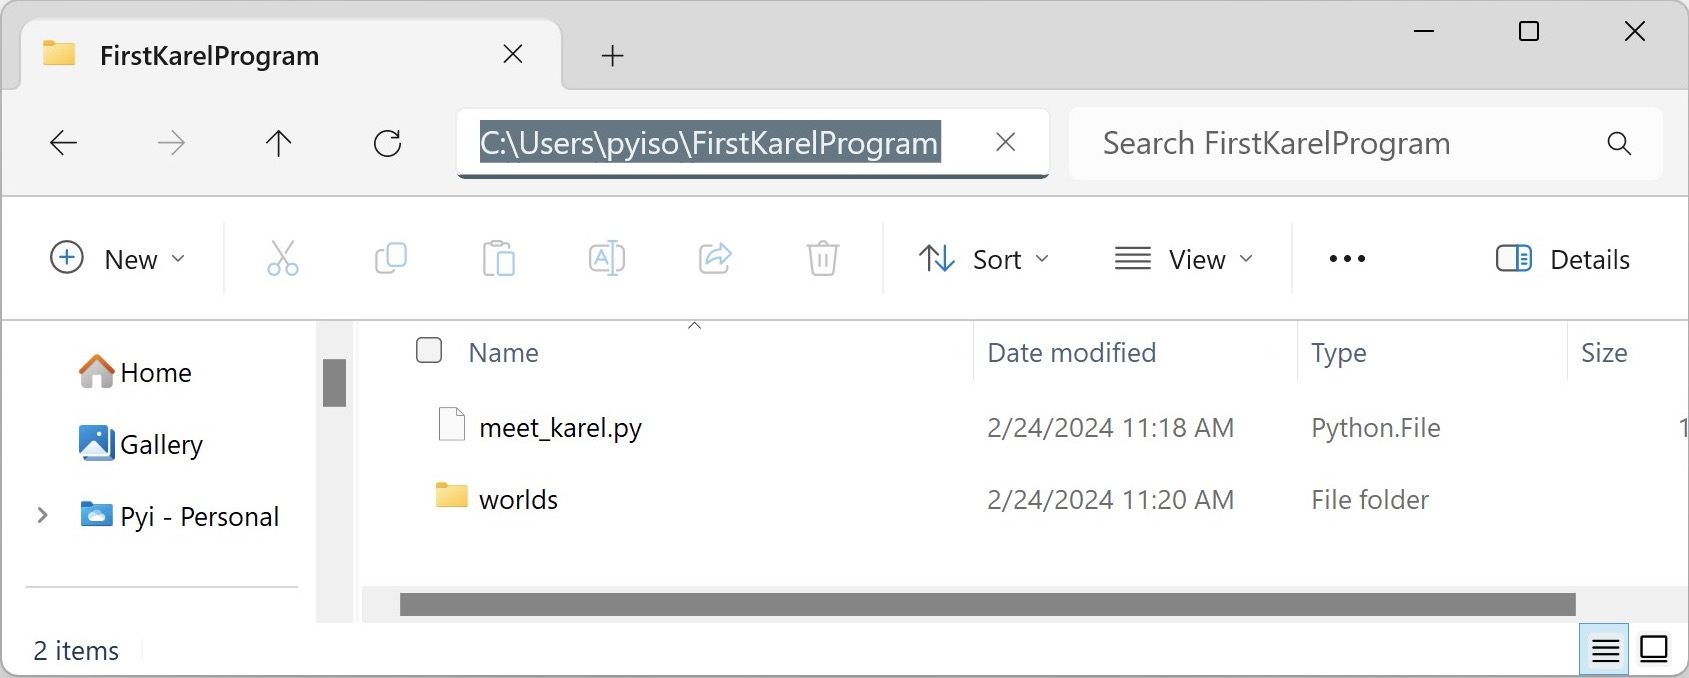
\includegraphics[width=.98\textwidth, trim={2.4mm 2mm 2mm 2mm},clip]{images/ch01/projstruct.jpg}};
    \drawshadow{image}
\end{tikzpicture}
\caption{} 
\label{fig:projstruct}
\end{figure}

\begin{figure}[tbh!]
\begin{tikzpicture}
    \node[anchor=south west,inner sep=0] (image) at (0,0)
        {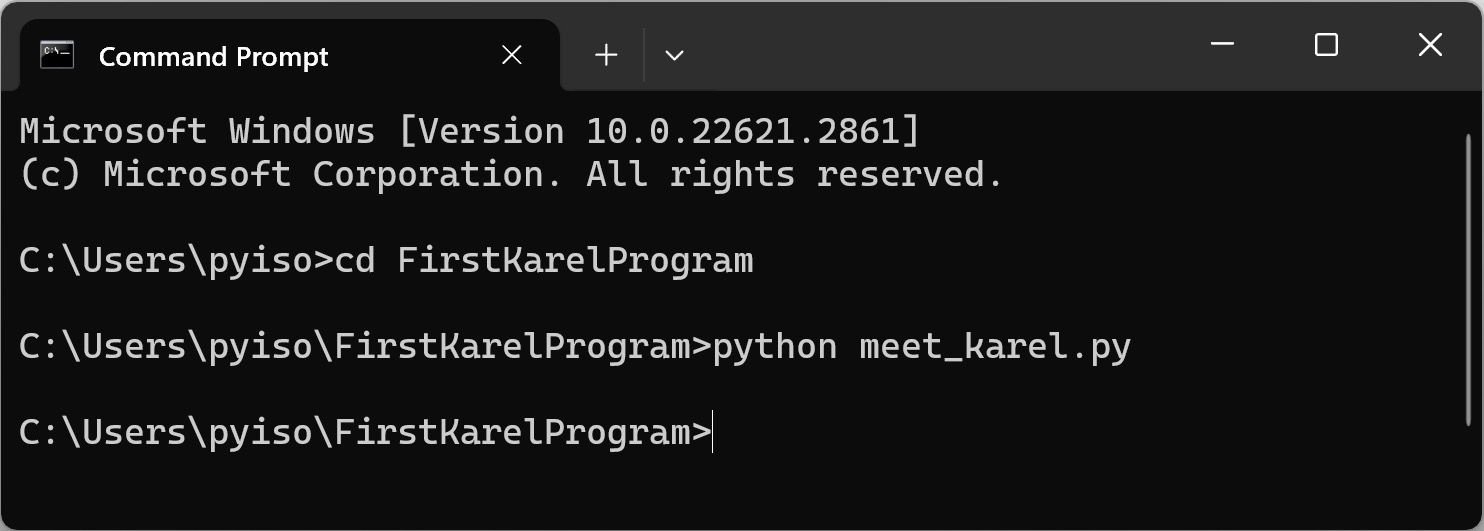
\includegraphics[width=.98\textwidth, trim={2.4mm 2mm 2mm 2mm},clip]{images/ch01/runkrl.jpg}};
    \drawshadow{image}
    \draw [draw=red, thick,rounded corners] (2.825,2.58) rectangle (6.65,2);
    \draw [draw=red, thick,rounded corners] (6.1,1.83) rectangle (10,1.25);

\end{tikzpicture}
\caption{} 
\label{fig:runkrl}
\end{figure}

\begin{figure}[tbh!]
\begin{tikzpicture}
    \node[anchor=south west,inner sep=0] (image) at (0,0)
        {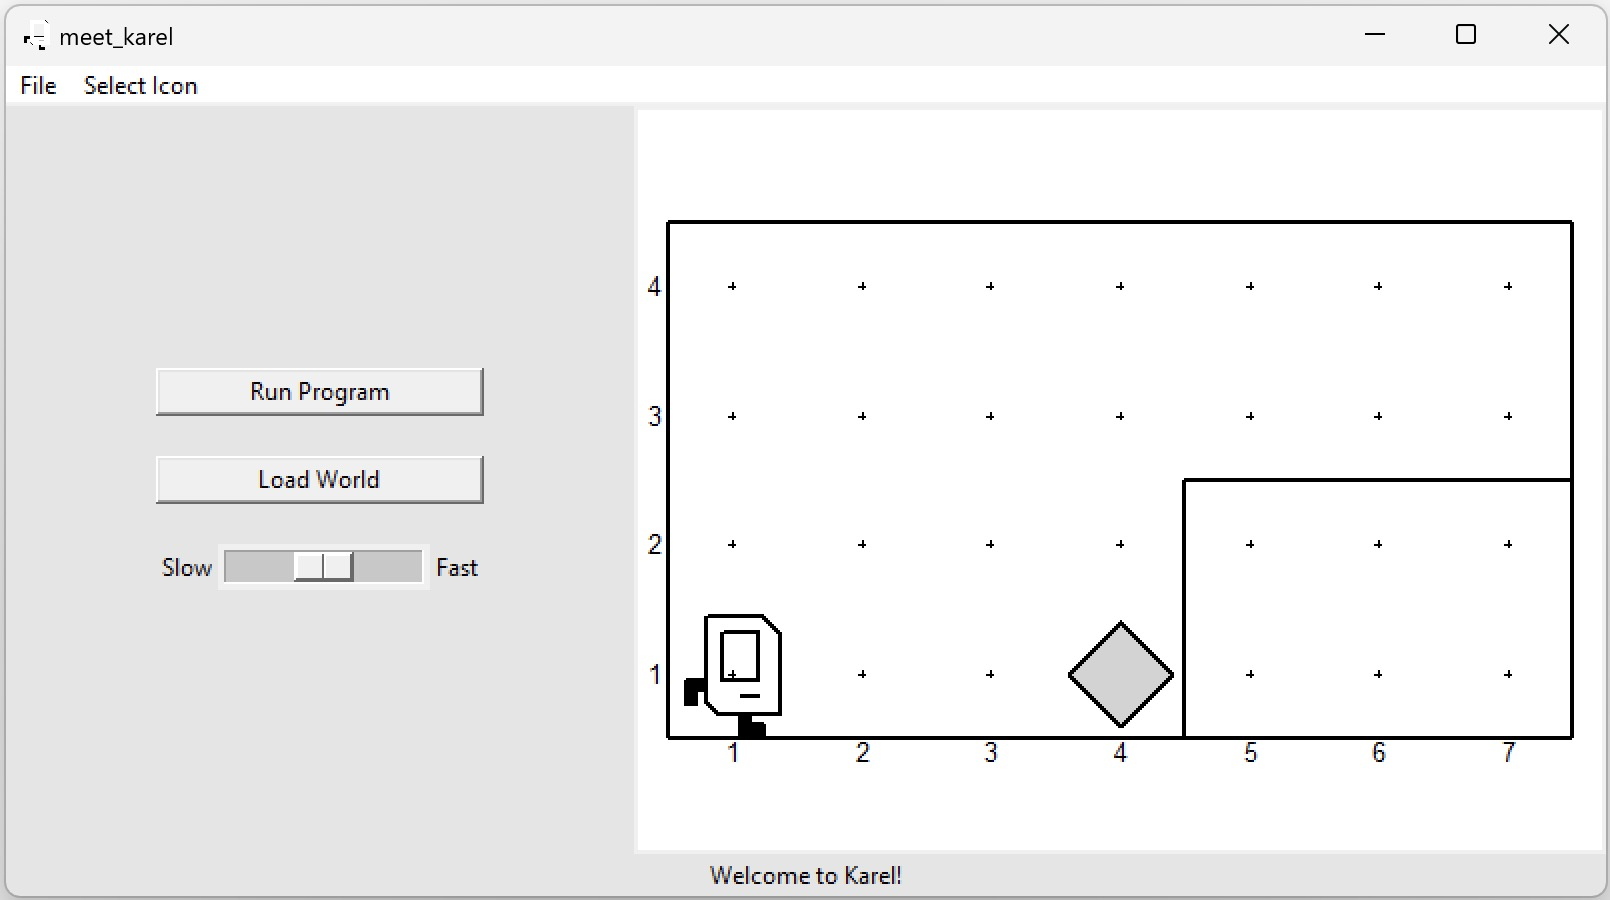
\includegraphics[width=.98\textwidth, trim={2.4mm 2mm 2mm 2mm},clip]{images/ch01/mtkrlprgm.jpg}};
    \drawshadow{image}
\end{tikzpicture}
\caption{} 
\label{fig:mtkrlprgm1}
\end{figure}

\section{Move Beeper to Other Side}
ပရိုဂရမ်းမင်း လေ့လာတဲ့အခါ စာချည်းပဲ ဖတ်နေပြီး အမှန်တကယ် နားလည်သွားဖို့ဆိုတာ မဖြစ်နိုင်ပါဘူး။ လက်တွေ့ စမ်းသပ်ကြည့်၊ ရေးကြည့်မှပဲ တကယ် နားလည်လာမယ်။ တကယ်လည်း ကျွမ်းကျွမ်းကျင်ကျင် ရေးတတ်လာမှာပါ။ ဒါကြောင့် လက်တွေ့ရေးကြည့်ပါ။ များများ လေ့ကျင့်ပါ။ ဥပမာတွေကိုလည်း နားလည်အောင် ဖတ်ပြီးရင် မိမိဘာသာ အလွတ် ပြန်ရေးကြည့်ပါ။ 

ပုံ (\fRefNo{\ref{fig:mbtos}}) မှ ဘိပါကို နံရံအခြားတစ်ဘက် အောက်ခြေကို ရွှေ့ပေးတဲ့ ပရိုဂရမ် ရေးကြည့်ပါ။ \fEn{Python} ထုံးစံအရ \fEnSnd{move\_beeper\_to\_other\_side.py} ဖိုင်နဲ့ သိမ်းသင့်ပါတယ်။\fEnSnd{meet\_karel.zip} ဖိုင်ထဲမှာပါတဲ့ \fEnSnd{worlds} ဖိုဒါမှာပဲ အခု ကမ္ဘာဖိုင် ထည့်ပေးထားပါတယ်။ \fEnSnd{move\_beeper\_to\_other\_side.w} နံမည်နဲ့ပါ။ အန်ထရီပွိုင့်အတွက် အခုလိုရေးရပါမယ်။

\setlength{\fboxsep}{0pt}
\begin{minted}[frame=\mintframe, framerule=\mintrule,framesep= \mintsep, xleftmargin=\xlftmargin
    , bgcolor=mintbgcolor,rulecolor=mintrulecolor
    , python3=true,escapeinside=ßß]{python}
if __name__ == "__main__":
    run_karel_program("move_beeper_to_other_side")
\end{minted}

\begin{figure}[tbh!]
\begin{tikzpicture}
    \node[anchor=south west,inner sep=0] (image) at (0,0)
        {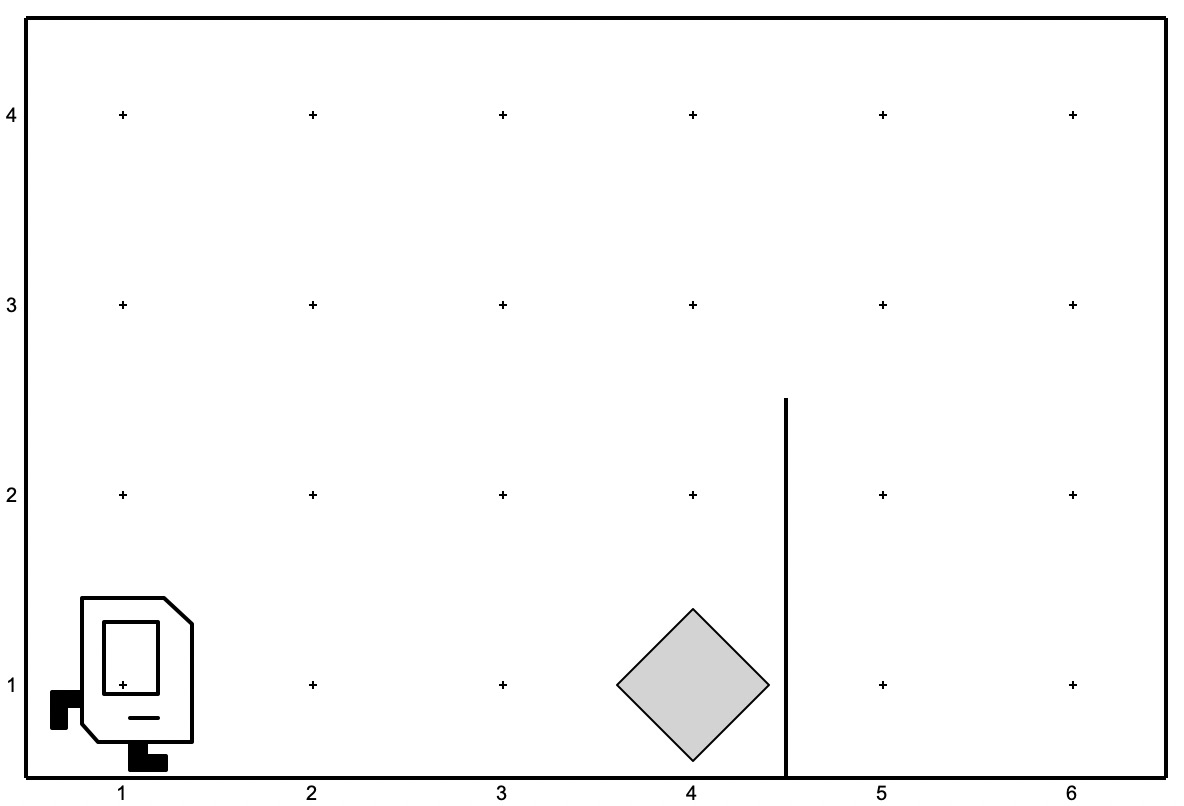
\includegraphics[width=3.5in, trim={2.4mm 2mm 2mm 2mm},clip]{images/ch01/MoveBeeperToOtherSide.jpg}};
    
\end{tikzpicture}
\caption{} 
\label{fig:mbtos}
\end{figure}


%

%

%
%
%
%အထက်ဖော်ပြပါ ပရိုဂရမ်ကုဒ် ပထမဆုံးတစ်ကြောင်းဟာ \fCode{import} စတိတ်မန့် ဖြစ်ပါတယ်။ ပရိုဂရမ်ကုဒ်ထဲမှာ ကလပ်စ် \fEn{(Class)} တစ်ခုကို ရည်ညွှန်းအသုံးပြုလို့ရအောင် \fCode{import} လုပ်ပေးရတာပါ။
%%
%\begin{minted}[frame=lines, framerule=0pt]{java}
%import stanford.karel.Karel;
%\end{minted}
%%
% \fCode{stanford.karel} \fOpn{ပက်ကေ့ချ်} \fEn{(package)} မှ \fCode{Karel} ကလပ်စ်ကို \fCode{import} လုပ်ထားတာ ဖြစ်တယ်။ စတိတ်မန့် အဆုံးမှာ ဆီမီးကော်လံ \fEn{(\fCode{;})} ပါတာကို သတိပြုပါ။ \fEn{Java} မှာ စတိတ်မန့် တစ်ကြောင်းဆုံးတိုင်း ဆီမီးကော်လံ ထည့်ပေးရပါမယ်။ \fOpn{ပက်ကေ့ချ်}ဆိုတာ ဆက်စပ်ရာ ကလပ်စ်တွေ စုစည်းထားတဲ့ ယူနစ်တစ်ခုပါပဲ။ \fCode{stanford.karel} \fOpn{ပက်ကေ့ချ်}ထဲက ကလပ်စ်အားလုံးကို \fCode{import} လုပ်မယ်ဆိုရင် ဒီလိုရေးရတယ်။
%%
%\begin{minted}[frame=lines, framerule=0pt]{java}
%import stanford.karel.*;
%\end{minted}
%%  
%လိုအပ်တဲ့ ကလပ်စ်ကိုပဲ ရွေးပြီး \fCode{import} လုပ်တာ ပိုကောင်းပါတယ်။
%
%\subsection*{ကလပ်စ်}
%ကလပ်စ် \fEn{(Class)} အကြောင်းကို နောက်ပိုင်းမှာ လေ့လာကြရမှာပါ။ အခုလောလောဆယ် ကလပ်စ်ကို ပရိုဂရမ်ကုဒ် စထရက်ချာတစ်မျိုးဟု ယူဆပါ။ \fEn{Java} ပရိုဂရမ်တစ်ခုမှာ အနည်းဆုံး ကလပ်စ်တစ်ခု ရှိရပါမယ်။ ကလပ်စ်တစ်ခုဖြစ်ဖို့အတွက် ဆင်းတက်စ်အရ အနည်းဆုံးရှိရမဲ့ ပုံစံက ဒီလိုပါ။
%%
%\begin{minted}[frame=lines, framerule=0pt]{java}
%public class MeetKarel {
%
%}
%\end{minted}
%% 
%ကလပ်စ်နံမည်က \fCode{MeetKarel} ဖြစ်ပါတယ်။ စကားလုံးအားလုံး အကြီးစာလုံးနဲ့ စထားတာ သတိထားကြည့်ပါ။ \fCode{meetkarel} လို့ရေးတာထက်  \fCode{MeetKarel} က စကားလုံးတစ်လုံးချင်းကို ပိုပြီးထင်ရှားစေတယ်။ ဒါကြောင့် အကြီးနဲ့စတဲ့ နည်းကိုပဲ အကြံပြုပါတယ်။
%
%\subsection*{\fSubSecCodeBf{Karel} ကလပ်စ်ကို \fSubSecCodeBf{extends} လုပ်ခြင်း}
%ရှေ့မှာတွေ့ခဲ့တဲ့ \fCode{MeetKarel} ကလပ်စ်ဟာ ကလပ်စ်အခွံချည်း ဖြစ်တယ်။ တွန့်ကွင်း အဖွင့်အပိတ်ကြားဟာ အလွတ်ဖြစ်နေပြီး ဘာပရိုဂရမ်ကုဒ်မှ မပါသေးပါဘူး။ ဒီကလပ်စ်ကို ကားရဲလ်ပရိုဂရမ်ဖြစ်အောင် အခုလိုရေးရပါမယ်။
%%
%\begin{minted}[frame=lines, framerule=0pt]{java}
%import stanford.karel.Karel;
%
%public class MeetKarel extends Karel {
%    
%}
%\end{minted}
%%
%\fCode{MeetKarel} ကလပ်စ်ဟာ \fCode{Karel} ကလပ်စ်ကို \fCode{extends} လုပ်ထားပါတယ်။ ပရိုဂရမ်ကုဒ်မှာ \fCode{Karel} ကလပ်စ်ကို ရည်ညွှန်းအသုံးပြုနိုင်ဖို့ အပေါ်မှာ \fCode{import} လုပ်ထားရတာပါ။ အခုအတိုင်းပဲ \fCode{MeetKarel}  ကို \fEn{IntelliJ} မှာ \fEn{run} ကြည့်ရင် ပုံ (\fRefNo{\ref{fig:meet_karel_window}}) မှာပြထားတဲ့ ကားရဲလ်ပရိုဂရမ် \fEn{window} တက်လာတာ တွေ့ရမှာပါ။ အဲဒီလိုမျိုး ကားရဲလ်ကမ္ဘာနဲ့ ဂရပ်ဖစ် \fEn{window} စခရင်ပေါ်မှာ ပေါ်လာတာဟာ  \fCode{Karel} ကလပ်စ်ထဲမှာ ပရိုဂရမ် ရေးပေးထားတဲ့ အတွက်ကြောင့် ဖြစ်တယ်။
%
%မှတ်ချက်။\qquad ။ အခုကစပြီး စာချည်းပဲဖတ်မနေဘဲ လက်တွေ့ပါ လိုက်လုပ်ကြည့်ဖို့ အလေးအနက် အကြံပြုချင်ပါတယ်။ စာမျက်နှာ \fRefNo{\pageref{apdx1}} နောက်ဆက်တွဲ (က) မှာ ဖော်ပြထားတဲ့အတိုင်း လိုအပ်တဲ့ ဆော့ဖ်ဝဲတွေထည့်သွင်းပါ။ နမူနာပါတဲ့ \fCode{MeetKarel} ပရိုဂရမ်ကို \fEn{run} ကြည့်ပါ။ 
%
%\begin{figure}[tb!]
%\begin{tikzpicture}
%    \node[anchor=south west,inner sep=0] (image) at (0,0)
%        {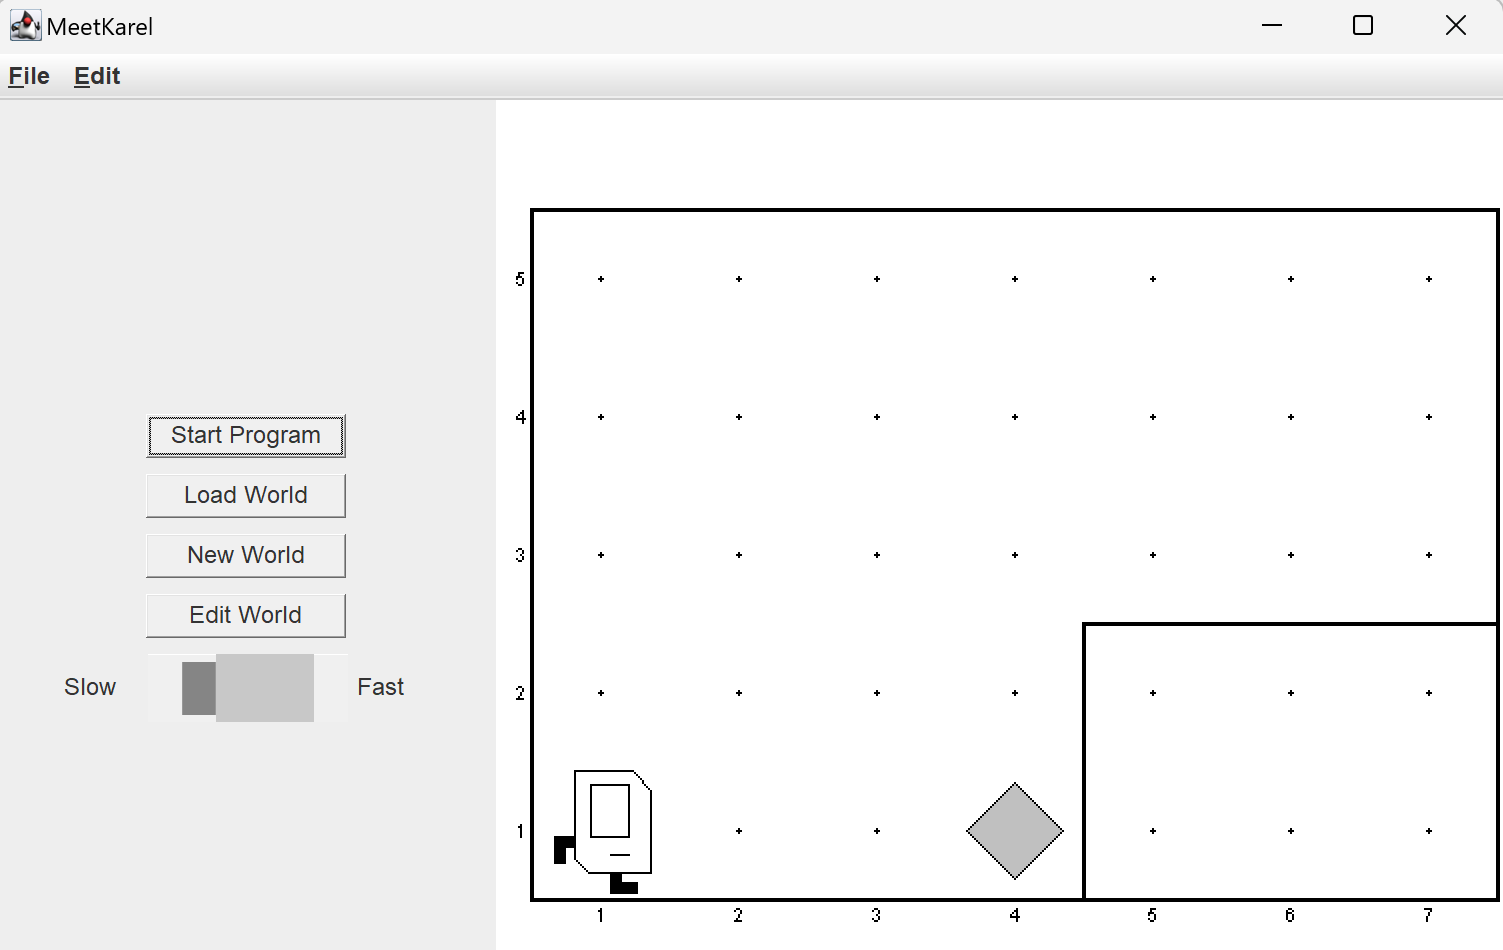
\includegraphics[width=.9\linewidth]{images/intellij_proj_create/MeetKarel.png}};
%    \drawshadow{image}
%\end{tikzpicture}
%\caption{}
%\label{fig:meet_karel_window}
%\end{figure}
%
%\subsection*{\fSubSecCodeBf{run} မက်သဒ်}
%
%မက်သဒ်ဆိုတာ စတိတ်မန့်တစ်စုကို ယူနစ်တစ်ခုအနေနဲ့ ဖွဲ့စည်းထားဖို့ အသုံးပြုတဲ့ စထရက်ချာတစ်မျိုးပါပဲ။ \fCode{move} စတိတ်မန့် သုံးခုကို ယူနစ်တစ်ခုအဖြစ် စုဖွဲ့ပေးထားတဲ့ \fCode{run} မက်သဒ်ကို အခုလိုတွေ့ရပါမယ်။ 
%%
%\begin{minted}[frame=lines, framerule=0pt]{java}
%import stanford.karel.Karel;
%
%public class MeetKarel extends Karel {
%    public void run() {
%        move();
%        move();
%        move();
%    }
%}
%\end{minted}
%%
%\fCode{run} မက်သဒ်ဟာ ကလပ်စ်ဘော်ဒီထဲမှာ ရှိရပါမယ်။ \fCode{run} ကို ဘယ်သူမဆို သုံးလို့ရအောင် \fCode{public} မက်သဒ်အနေနဲ့ သတ်မှတ်ထားတယ်။ \fCode{run} ဟာ \fCode{void} မက်သဒ်လည်းဖြစ်တယ်။ ဘာတန်ဖိုးမှ ပြန်ထုတ်မပေးတဲ့ မက်သဒ်လို့ အဓိပ္ပါယ်ရတယ်။  မက်သဒ်နံမည် \fCode{run} ဘေးမှာ ဝိုက်ကွင်းတစ်စုံပါရမယ်။ တွန့်ကွင်းတစ်စုံကတော့ မက်သဒ်ဘော်ဒီ အစနဲ့အဆုံးကို သတ်မှတ်ပေးထားတာ။ မက်သဒ်ဘော်ဒီထဲမှာ သက်ဆိုင်တဲ့ စတိတ်မန့်တွေ ရေးပေးရမယ်။ မက်သဒ်တွေအကြောင်း တစ်ခန်းသတ်သတ် လေ့လာကြရမှာပါ။ အဲဒီကျရင် အခုသိပ်နားမလည်တာတွေ အားလုံးရှင်းသွားပါလိမ့်မယ်။
%
%\fCode{run} ဟာ ကားရဲလ်ပရိုဂရမ်တွေအတွက် အထူးစီမံထားတဲ့ မက်သဒ်တစ်ခု ဖြစ်တယ်။ ပုံ (\fRefNo{\ref{fig:meet_karel_window}}) ကားရဲလ်ပရိုဂရမ် \fEn{window} ပေါ်လာပြီး \fEn{“Start Program”} နှိပ်လိုက်ရင် \fCode{run} မက်သဒ်ကို လုပ်ဆောင်ပေးတယ်။ \fEn{“Start Program”} မနှိပ်သေးရင် \fCode{run} နဲ့ဆိုင်တဲ့ စတိတ်မန့်တွေကလည်း အလုပ်မလုပ်သေးပါဘူး။ နှိပ်လိုက်တော့မှ \fCode{run} က စပြီးအလုပ်လုပ်တာပါ။ \fEn{“Start Program”} နှိပ်တဲ့အခါတိုင်း \fCode{run} ကို လုပ်ဆောင်ပေးမှာပါ။ 
%
%\fCode{MeetKarel} ကို အပေါ်မှာ ပြထားတဲ့အတိုင်း \fEn{IntelliJ} မှာ ရေးပြီး \fEn{run} ကြည့်ပါ။ \fEn{“Start Program”} နှိပ်လိုက်ရင် ကားရဲလ်က ရှေ့ကို သုံးခါရွှေ့ပေးပါလိမ့်မယ်။ နောက်ထပ်တစ်ခါ ထပ်နှိပ်ရင် \fCode{run} ကလည်း တစ်ခါထပ် အလုပ်လုပ်မှာပါ။ ဒါပေမဲ့ ရှေ့မှာ နံရံပိတ်နေတဲ့အတွက် ရွှေ့လို့မရတော့ဘဲ အယ်ရာတက်ပါလိမ့်မယ်။ \fEn{“Load World”} ကို နှိပ်ပြီး \fEn{MeetKarel.w} ဖိုင်ကိုရွေးလိုက်ရင် နဂိုအနေအထားပြန်ဖြစ်သွားပါလိမ့်မယ်။ ဒါမှမဟုတ် ပရိုဂရမ်ကို ပိတ်ပြီး ပြန် \fEn{run} နိုင်ပါတယ်။
%
%\subsection*{မက်သဒ်ကောလ် စတိတ်မန့်}
%\fCode{run} မက်သဒ်ထဲမှာတွေ့ရတဲ့ စတိတ်မန့်တွေဟာ မက်သဒ်ကောလ် \fEn{(method call)} စတိတ်မန့်တွေဖြစ်ပါတယ်။ \fCode{move}\fEn{,} \fCode{pickBeeper}\fEn{,}  \fCode{putBeeper}\fEn{,} \fCode{turnLeft} ကွန်မန်းတွေဟာ \fCode{Karel} ကလပ်စ်မှာ သတ်မှတ်ပေးထားတဲ့ မက်သဒ်တွေဖြစ်တယ်။ ပရိုဂရမ်ရေးတဲ့အခါ ကားရဲလ်ကွန်မန်းတွေကို မက်သဒ်ကောလ် စတိတ်မန့်အနေနဲ့ ရေးရမယ်။ ဥပမာ ဘယ်ဘက် လှည့်ခိုင်းတာကို
%%
%\begin{minted}[frame=lines, framerule=0pt]{java}
%turnLeft();
%\end{minted}
%%
%လို့ ရေးရပါမယ်။ စတိတ်မန့်ဖြစ်တဲ့အတွက် ဆီမီးကော်လံချပေးရမှာ ဂရုပြုပါ။ 
%
%\subsection*{မှတ်ချက်ရေးခြင်း}
%ဘိပါကို နေရာရွှေ့ထားဖို့ အပြီးထိဆက်ရေးထားတဲ့ ပရိုဂရမ်ကို အောက်မှာ ပြန်ဖော်ပြပေးထားပါတယ်။ မှတ်ချက် \fEn{(comment)} ရေးထားတာ တချို့ ပါနေတာကလွဲရင် စာမျက်နှာ \fRefNo{\pageref{lst:MeetKarel1}} မှာ ဖော်ပြခဲ့တဲ့ ပရိုဂရမ်နဲ့ တူတူပါပဲ။
%%
%\begin{minted}[frame=lines, framerule=0pt]{java}
%/* 
%This is our first example Karel program. This program is for 
%moving the beeper to(5,3) corner.
%*/
%import stanford.karel.Karel;
%
%public class MeetKarel extends Karel {
%    public void run() {
%        move();
%        move();
%        move();
%        pickBeeper();
%        turnLeft();
%        move();
%        move();
%        // we want karel to turn right
%        // turning left 3 times is the same as turning right
%        turnLeft();
%        turnLeft();
%        turnLeft();
%        move();
%        putBeeper();
%    }
%}
%\end{minted}
%% 
%ကွန်းမန့်ရေးချင်ရင် \fCode{/*} နဲ့ \fCode{*/} အတွင်း သို့မဟုတ် \fCode{//} နောက်မှာ ရေးရပါတယ်။ ကွန်းမန့်တွေကို ပရိုဂရမ်ကုဒ်အနေနဲ့ မယူဆရပါဘူး။ တနည်းအားဖြင့် ကွန်းမန့်တွေဟာ ကွန်ပျူတာ ဆောက်ရွက်ပေးရမဲ့ ညွှန်ကြားချက်တွေ မဟုတ်ပါဘူး။ ပရိုဂရမ်ကုဒ်ကို နားလည်အောင်ရှင်းပြတာ သို့မဟုတ် ဘယ်လိုစဉ်းစားပြီး ရေးခဲ့တာလည်း နောင်တချိန်ပြန်ဖတ်တဲ့အခါ မှတ်မိအောင် ပရိုဂရမ်ကုဒ်ထဲမှာ ကွန်းမန့်ရေးထားရလေ့ရှိပါတယ်။
%
%\fCode{/*} နဲ့ \fCode{*/} အတွင်း ရေးထားတဲ့ စာကြောင်းအားလုံးကို ကွန်းမန့်အနေနဲ့ယူဆတယ်။ \fEn{Multiline comment} အတွက် သုံးတာဖြစ်တယ်။ ဥပမာ
%%
%\begin{minted}[frame=lines, framerule=0pt]{java}
%/*
%This is the first line of comment.
%This is the second line of comment
%*/
%\end{minted}
%%
%\fCode{//} ကတော့ နောက်မှာရှိတဲ့ စာကြောင်းကိုပဲ ကွန်းမန့်အနေနဲ့ ယူဆတာ။ ဥပမာ
%%
%\begin{minted}[frame=lines, framerule=0pt]{java}
%pickBeeper(); // to pick the beeper at the current corner if any
%turnLeft();
%\end{minted}
%%
%ဒီနှစ်ကြောင်းမှာ \fCode{pickBeeper} နဲ့ \fCode{turnLeft} စတိတ်မန့်တွေဟာ ကွန်းမန့်မဟုတ်ပါ။  ပထမတစ်ကြောင်း နောက်ပိုင်း စာလုံးအစောင်းနဲ့ စာသားတွေကပဲ ကွန်းမန့်ဖြစ်ပါတယ်။  
%%
%\begin{minted}[frame=lines, framerule=0pt]{java}
%pickBeeper(); // to pick the beeper at the current corner if any
%// turnLeft();
%\end{minted}
%%
%ဒီလိုဆိုရင်တော့ ဒုတိယအကြောင်း \fCode{turnLeft} ကလည်း ကွန်းမန့်ဖြစ်သွားပါမယ်။
%
%\section{လေ့ကျင့်ရန် ပရိုဂရမ်}
%အခြားအခြားသော ပညာရပ်တွေလိုပဲ ပရိုဂရမ်ရေးတာဟာလည်း စာဖတ်နေရုံနဲ့ ကျွမ်းကျင်တတ်မြောက်သွားမဲ့ ပညာရပ်မျိုး မဟုတ်ပါဘူး။ လက်တွေ့ရေးပြီး အချိန်ပေး လေ့ကျင့်ဖို့ လိုအပ်တယ်။ များများရေး များများလေ့ကျင့်မှ ကျွမ်းကျင်လာမယ်။ ဒီအတွက် လိုအပ်တဲ့ ဆော့ဖ်ဝဲတွေ ထည့်ထားရပါမယ်။ စာမျက်နှာ \fRefNo{\pageref{apdx1}} နောက်ဆက်တွဲ (က) ကိုဖတ်ပြီး ဆော့ဖ်ဝဲတွေ သွင်းပါ။ ပရောဂျက်အသစ်၊ ကလပ်စ်အသစ် ဖန်တီးနည်းတို့ကိုလည်း နောက်ဆက်တွဲ (က) မှာ အသေးစိတ်ဖော်ပြပေးထားပါတယ်။ အခုပဲ သွားဖတ်ပြီး လက်တွေ့လိုက်လုပ်ပါလို့ အကြံပြုချင်ပါတယ်။
%
%ဒီအခန်းအတွက် နမူနာပရောဂျက် ထည့်ပြီးသွားရင် နောက်ဆက်တွဲ (က) စာမျက်နှာ \fRefNo{\pageref{apdx1:new_class}} မှာ ဖော်ပြထားတဲ့အတိုင်း ကလပ်စ်အသစ်ဖန်တီးယူပါ။ ပုံမှာတွေ့ရတဲ့ ဘိပါကို နံရံအခြားတစ်ဘက် မြှားပြထားတဲ့နေရာကို ရွှေ့ပေးတဲ့ ပရိုဂရမ် ရေးပါ။
%
%\begin{figure}[htb!]
%\begin{tikzonimage}[width=4in]{images/ch01/MoveBeeperToOtherSide.jpg}%[tsx/show help lines]
%    \draw[-{Latex[length=3mm]}] (0.85 ,0.27)--(0.75, 0.16);
%\end{tikzonimage}
%\caption{\fCptCodeBf{MoveBeeperToOtherSide} ကမ္ဘာ}
%\label{fig:move_beeper_to_other_side1}
%\end{figure}
%
%\subsection*{ကားရဲလ်ကမ္ဘာ ဖိုင် (Karel's World File)}
%ဒီပရိုဂရမ်အတွက် ကလပ်စ်နံမည်ကို \fCode{MoveBeeperToOtherSide} ပေးပါလို့ ပြောထားတာ အကြောင်းရှိပါတယ်။ အမှန်က ကားရဲလ်ပရိုဂရမ်တစ်ခုမှာ သင့်တော်တဲ့ ကလပ်စ်နံမည် စိတ်ကြိုက်ရွေးချယ် ပေးလို့ရပါတယ်။ ဒါပေမဲ့ ပရိုဂရမ် \fEn{run} လိုက်ရင် ပေါ်လာတဲ့ကမ္ဘာက အခုပုံမှာတွေ့ရတာနဲ့ တူမှာမဟုတ်ဘူး။ အခုပြထားတဲ့ကမ္ဘာပုံဖြစ်အောင် \fEn{worlds} ဖိုဒါထဲက \fEn{MoveBeeperToOtherSide.w} ဖိုင်မှာ သတ်မှတ်ပေးထားရတာပါ။ \fCode{MeetKarel} ကမ္ဘာပုံဖြစ်အောင် အဲ့ဒီဖိုဒါထဲကပဲ \fEn{MeetKarel.w} မှာ သတ်မှတ်ပေးထားတာ။ ကားရဲလ်ပရိုဂရမ် ကလပ်စ်တစ်ခုကို \fEn{run} တဲ့အခါ ကလပ်စ်နံမည်နဲ့ တူတဲ့ \fEnEmpBf{.w} ဖိုင်ကိုရှာပြီး အဲဒီဖိုင်မှာသတ်မှတ်ထားတဲ့ ကမ္ဘာကို တင်ပေးတာပါ။ နံမည်တူရှာမတွေ့ရင်တော့ \(10 \times 10\) အရွယ် \fEn{default} ကမ္ဘာကို  တင်ပေးမှာပါ။ \fEn{“Load World”} နှိပ်ပြီး \fEn{worlds} ဖိုဒါထဲက လိုချင်တဲ့ ကမ္ဘာကို ခေါ်တင်လို့ရတယ်။ ပရိုဂရမ် \fEn{run} လိုက်၊ လိုချင်တဲ့ကမ္ဘာကို ခေါ်တင်လိုက်နဲ့ ကရိကထများမယ်။ ဒါကြောင့် ကမ္ဘာနံမည်နဲ့ ကလပ်စ်နံမည် တူအောင်ပေးခိုင်းရတာ ဖြစ်တယ်။
%
%\section{ဖြစ်လေ့ရှိတဲ့ အမှားတချို့}
%
%အခုမှ ပရိုဂရမ်စရေးဖူးတဲ့ လူသစ်တွေ ဖြစ်လေ့ရှိတဲ့ အမှားတချို့ကို ဆက်လက်ဖော်ပြပါမယ်။
%
%\subsection*{တွန့်ကွင်းကျန်ခဲ့ခြင်း}
%ကလပ်စ်ဘော်ဒီ၊ မက်သဒ်ဘော်ဒီတို့ရဲ့ အစ အဆုံးကို တွန့်ကွင်း အဖွင့် အပိတ်နဲ့ သတ်မှတ်ပေးရတာပါ။ အဖွင့် သို့မဟုတ် အပိတ် တွန့်ကွင်း ကျန်ခဲ့ရင် ဆင်းတက်စ်အမှားဖြစ်ပြီး ပရိုဂရမ်ကို \fEn{run} လို့ရမှာ မဟုတ်ပါဘူး။ အပြင်ဆုံးမှာ ကလပ်စ်ဘော်ဒီအတွက် တွန့်ကွင်းတစ်စုံ၊ ကလပ်စ်ဘော်ဒီထဲက \fCode{run} မက်သဒ်ဘော်ဒီအတွက် တွန့်ကွင်းတစ်စုံ ရှိရမှာဖြစ်တယ်။
%
%အဖွင့်အပိတ် မစုံရင် \fEn{IntelliJ} က ကုဒ်ရေးတဲ့ \fEn{editor} မှာရော ပရောဂျက်ဖိုဒါမှာပါ အယ်ရာပြပေးပါတယ်။ တွန့်ကွင်းကျန်ခဲ့လို့ ဖြစ်တာဆိုရင် ဖြည့်ပေးလိုက်ရင် အယ်ရာတွေမပြတော့ပါဘူး။ ဆက်ပြနေသေးရင် အခြားအကြောင်းကြောင့်ဖြစ်တာ ဖြစ်နိုင်ပါတယ်။
%
%\subsection*{ဆီမီးကော်လံ ကျန်ခဲ့ခြင်း}
%\fCode{import} စတိတ်မန့်၊ မက်သဒ်ကောလ်စတိတ်မန့် တွေမှာ ဆီမီးကော်လံနဲ့ ဆုံးပေးရပါမယ်။ ကျန်ခဲ့ရင် ဆင်းတက်စ်အယ်ရာဖြစ်ပြီး \fEn{run} လို့ရမှာ မဟုတ်ပါ။ 
%
%\subsection*{ဝိုက်ကွင်းကျန်ခဲ့ခြင်း}
%\fCode{run} မက်သဒ်သတ်မှတ်ချက်မှာ ဝိုက်ကွင်းအဖွင့်အပိတ် တစ်စုံပါရမယ်။ မက်သဒ်ကောလ် စတိတ်မန့်တွေမှာလည်း ဝိုက်ကွင်းတစ်စုံ ပါရပါမယ်။
%
%\subsection*{စာလုံးအကြီးအသေး၊ စာလုံးပေါင်းနှင့် နံမည်ပေးခြင်း}
%\fEn{Java} မှာ နံမည်တွေ စာလုံး အကြီးအသေး လွဲလို့မရပါဘူး။ \fEn{“Case Sensitive”} ဖြစ်တယ်လို့ ခေါ်ပါတယ်။ မက်သဒ်ကောလ်လုပ်တဲ့ စတိတ်မန့်တွေမှာ စာလုံးပေါင်းရော အကြီးအသေးပါ ဂရုစိုက်ရေးဖို့လိုပါတယ်။ ဥပမာ ဒီလိုတွေရေးရင် အယ်ရာဖြစ်မှာပါ။
%%
%\begin{minted}[frame=lines, framerule=0pt,escapeinside=ßß]{text}
%turnleft();    //ß l \fMM{အသေးဖြစ်နေ}ß 
%PickBeeper();  //ß P \fMM{အကြီးဖြစ်နေ}ß 
%turn Left();   //ß \fMM{စပေ့စ်ပါနေတယ်}ß
%\end{minted}
%% 
%\fEn{IntelliJ} ရဲ့ \fEn{Code Completion} ဖီချာက ဒီလိုအမှားမျိုးနည်းအောင် ကူညီပေးပါတယ်။
%
%နံမည်ပေးတာရယ်၊ ပေးထားတဲ့နံမည်နဲ့ ရည်ညွှန်းအသုံးပြုတာရယ် ကိစ္စနှစ်ခုကို ခွဲခြားပြောဖို့လိုပါတယ်။ ကလပ်စ်သတ်မှတ်တဲ့အခါနဲ့ မက်သဒ်သတ်မှတ်တဲ့အခါမှာ ကလပ်စ်နံမည်၊ မက်သဒ်နံမည် ပေးရပါတယ်။ နံမည်ပေးတဲ့အခါ လိုက်နာဖို့ လိုအပ်တာတွေရှိပါတယ်။ နံမည်က ဂဏန်းနဲ့စလို့မရပါဘူး။ နံမည်မှာ စပေ့စ်ပါလို့မရဘူး။ ဥပမာ ဒီလိုတွေမရပါဘူး။
%%
%\begin{minted}[frame=lines, framerule=0pt,escapeinside=ßß]{java}
%public class ß\color{blue}\fCodeBf{1stKarelExample}ß ß\fCode{\bropn ...}ß 
%\end{minted}
%%
%%
%\begin{minted}[frame=lines, framerule=0pt,escapeinside=ßß]{java}
%public class ß\color{blue}\fCodeBf{Meet Karel}ß ß\fCode{\bropn ...}ß
%\end{minted}
%%
%ဒါကနံမည်ပေးတဲ့အခါ လိုက်နာဖို့လိုတဲ့ စည်းမျဉ်းတချို့ပါ။ အသေးစိတ်ကို နောက်ပိုင်းမှာ ဆက်လေ့လာရမှာပါ။ 
%
%နောက်တစ်ခုက နံမည်နဲ့ ရည်ညွှန်းအသုံးပြုတာပါ။ \fCode{turnLeft} မက်သဒ်ကို \fCode{Karel} ကလပ်စ်ထဲမှာ သတ်မှတ်ထားတယ်လို့ ပြောခဲ့တယ်။ \fCode{turnLeft} နံမည်နဲ့ပဲ မက်သဒ်ကောလ် လုပ်ရပါမယ်။ ဒါဟာ မက်သဒ်နံမည်နဲ့ မက်သဒ်ကို ရည်ညွှန်းအသုံးပြုတာပါ။ ပေးထားတဲ့နံမည်အတိုင်း အတိအကျရေးပြီး ရည်ညွှန်းအသုံးပြုရပါမယ်။ လွဲလို့မရပါဘူး။ ကလပ်စ်နံမည်လည်း ထိုနည်းတူစွာပါပဲ။ \fCode{Karel} ကလပ်စ်ကို ရည်ညွှန်းအသုံးပြုတဲ့အခါ နံမည်စာလုံးပေါင်းတာ တိကျဖို့ လိုပါတယ်။
%
%\fCode{run} မက်သဒ်ကို \fCode{Run} လို့နံမည်ပေးမိရင်လည်း ပြဿနာရှိပါတယ်။ \fEn{“Start Program”} နှိပ်ရင် \fCode{run} (စာလုံးအသေး) နံမည်နဲ့ မက်သဒ်ကို လုပ်ဆောင်ပေးတာပါ။ \fCode{Run} ဖြစ်နေရင် အဲ့ဒီမက်သဒ်က အလုပ်လုပ်မှာ မဟုတ်ပါဘူး။